\documentclass[a4paper,12pt]{article}
\usepackage{outline}
\usepackage{pmgraph}
\usepackage[normalem]{ulem}
\usepackage{comment} % enables the use of multi-line comments (\ifx \fi)
\usepackage{lipsum} %This package just generates Lorem Ipsum filler text.
\usepackage{fullpage} % changes the margin
\usepackage{listings}
\usepackage{color}
\usepackage{mdframed}
\usepackage{listings}
\usepackage{amssymb}
\usepackage{amsmath}
\usepackage{graphicx}
\graphicspath{ {../screenshots/} }
\renewcommand{\lstlistingname}{Code Block}% Listing -> Algorithm
\renewcommand{\lstlistlistingname}{List of \lstlistingname s}% List of Listings -> List of Algorithms

\linespread{1.5}
%--------------------Indention
\setlength{\parindent}{15pt}
\lstset{frame=shadowbox, rulesepcolor=\color{white}}
\mdfsetup{frametitlealignment=\center}
\lstset{
  numbers=left,
  stepnumber=1,
  firstnumber=1,
  numberfirstline=true
}

\begin{document}
\section*{Objective}

\hspace{15pt}In this lab, a fast-adder circuit for two-opperand addition was designed called carry-lookahead addition. The design consists of using a combination of dataflow and structural Verilog. The designs were then simulated on the Xilinx ISE to check for correctness. The propagation delays for for a 4-bit and 16-bit carry-lookahead adder were also analyzed in order to compare to similar sized ripple-carry adders.  

\section*{Design}

% EXP 1
% generate propagate unit
% carry lookahead unit
% summation unit
% carry lookahead 4bit
% 4-bit carry lookahead adder
% modified to 2ns gate delays - propagation was measuered
% \lstinputlisting[language=Verilog,,caption=4-Bit ALU ]{../code/code name.v}
% EXP 2
% block_carry_lookahead_unit.v
% \lstinputlisting[language=Verilog,,caption=4-Bit ALU ]{../code/block_carry_lookahead_unit.v}
% GPU and SU changed to be 16 bit wide with removed gate delay
% \lstinputlisting[language=Verilog,,caption=4-Bit ALU ]{../code/code name.v}
% top level module carry_lookahead_16bit
% \lstinputlisting[language=Verilog,,caption=4-Bit ALU ]{../code/code name.v}
% Edit test bennch TEST_DELAY (9ns)
% \lstinputlisting[language=Verilog,,caption=4-Bit ALU ]{../code/code name.v}

\textbf{Experiment 1}

To start off the experiment, the following code was written for the most part as part of the prelab. A few modifications were made into order to function properly. The first three blocks of code are of the modules (\textit{generate-propagate-unit, carry-lookahead-unit,} and \textit{summation-unit}) used in \textit{Code Block 4} for the top level   module \textit{carry-lookahead-4bit}

% Verilog code template
  \lstinputlisting[language=Verilog,,caption=Generate Propagate Unit (4-Bit)]{../code/generate_propagate_unit.v}

  \lstinputlisting[language=Verilog,,caption=Carry Lookahead Unit (4-Bit)]{../code/carry_lookahead_unit.v}
  
  \lstinputlisting[language=Verilog,,caption=Summation Unit (4-Bit)]{../code/summation_unit.v}
  
  \lstinputlisting[language=Verilog,,caption=Top Level Carry Lookahead (4-Bit)]{../code/carry_lookahead_4bit.v}
  
  For the next part, gate delays were modified in the following modules.
  
  \lstinputlisting[language=Verilog,firstnumber=8,firstline=8,lastline=9,caption=Generate Propagate Unit (4-Bit with Delay)]{../code/generate_propagate_unit_delay.v}

  \lstinputlisting[language=Verilog,firstnumber=8,firstline=8,lastline=14,caption=Carry Lookahead Unit (4-Bit with Delay)]{../code/carry_lookahead_unit_delay.v}
  
  \lstinputlisting[language=Verilog,firstnumber=8,firstline=8,lastline=8,caption=Summation Unit (4-Bit with Delay)]{../code/summation_unit_delay.v}

  \hspace{-15pt}\textbf{Experiment 2}
  
  In the next experiment, a block carry lookahead unit was designed. The module interface is as follows:

  \lstinputlisting[language=Verilog,,caption=Block Carry Lookahead Unit]{../code/block_carry_lookahead_unit.v}
  
  Next, the generate propegate unit and summation unit were modified in order to take in 15 bit wires as shown below. The gate delays were also removed.
  
  \lstinputlisting[language=Verilog,firstnumber=4,firstline=4,lastline=5,caption=Generate Propagate Unit (16-Bit)]{../code/generate_propagate_unit_delay.v}
  
  \lstinputlisting[language=Verilog,firstnumber=4,firstline=4,lastline=5,caption=Summation Unit (16-Bit)]{../code/summation_unit_delay.v}
  
  Finally the past modules were implemented into a top−level module for a 16-bit carry lookahead adder.
  
  \lstinputlisting[language=Verilog,,caption=16-Bit Carry Lookahead Adder]{../code/carry_lookahead_16bit.v}
  
\section*{Results}

% Figure with caption
% \begin{figure}[h]
%   \begin{center}
%     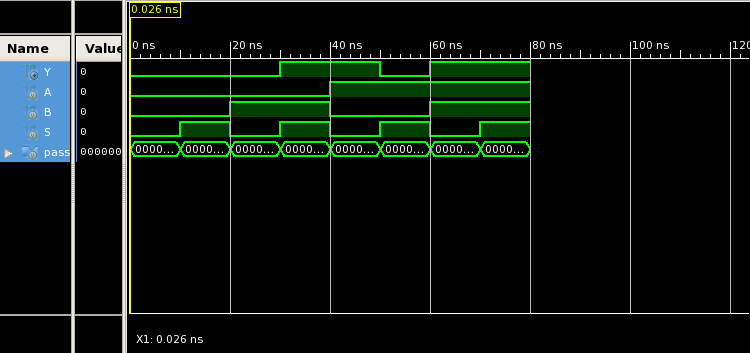
\includegraphics[scale=1]{2_1MuxPlot.png}
%     \caption{\textit{2-Bit 2:1 MUX Plots}}
%   \end{center}
% \end{figure}


\section*{Conclusion}


\section*{Questions}

\begin{enumerate}
  \item \textbf{Include the source code with comments for all odules in lab. you do not have to include test bench code. Code without comments will not be accepted!}
  \item \textbf{Include the simulation screenshots requested in the above experiments in addition to the corresponding test bench console output.}
  \item \textbf{Answer all questions throught the lab manual}
  \item \textbf{How does the gate-cout of the 16-bit carry-looahead adder compar to that of a ripple-carry adder of the same size.}
  \item \textbf{How does the progaagtion delay of the 4-bit carry-lookahead adder compare to that of a ripple-carry adder of the same size. Similarly, how does the 16-bit carry-lookahead adder compare to that of a ripple-carry adder of the same size.}
\end{enumerate}

\section*{Student Feedback}

\begin{enumerate}
  \item \textbf{What did you like most about the lab assignment and why? What did you like least about it and why?}
  \vspace{10pt}

  \item \textbf{Were there any section of the lab manual that were unclear? If so, what was unclear? Do you have any suggestions for improving the clarity?}
  \vspace{10pt}

  \item \textbf{What suggestions do you have to improve the overall lab assignment?}
  \vspace{10pt}

\end{enumerate}

\ifx
\begin{thebibliography}{1}
\bibitem{Verilog} Charles Kime \& Thomas Kaminski  \emph{Logic and Computer Design Fundamentals} \\ \hspace{15pt}\textit{http://www.cs.bilkent.edu.tr/~will/courses/CS223/Verilog/LCDF3_Verilog_Ch_4.pdf}
\end{thebibliography}

\section*{Attachments}
%Make sure to change these
Lab Notes, HelloWorld.ic, FooBar.ic
%\fi %comment me out

\begin{thebibliography}{9}
\bibitem{Verilog} Charles Kime & Thomas Kaminski  \emph{Logic and Computer Design Fundamentals} \textit{http://www.cs.bilkent.edu.tr/~will/courses/CS223/Verilog/LCDF3_Verilog_Ch_4.pdf}
\end{thebibliography}

%How to cite
Put your Problem statement here! Example of a Citation\cite[p.219]{Robotics}. Here's Another Citation\cite{Flueck}
\fi
\end{document}
